% Created by tikzDevice version 0.12
% !TEX encoding = UTF-8 Unicode
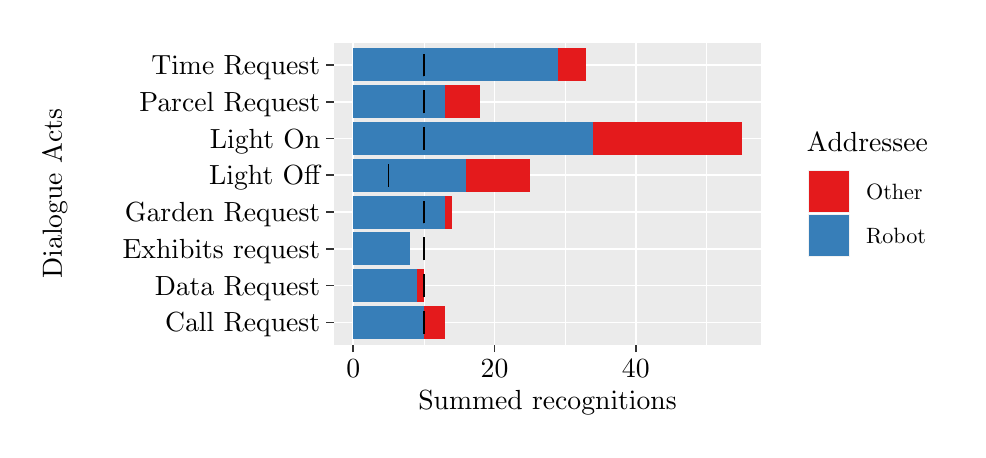
\begin{tikzpicture}[x=1pt,y=1pt]
\definecolor{fillColor}{RGB}{255,255,255}
\path[use as bounding box,fill=fillColor,fill opacity=0.00] (0,0) rectangle (336.00,145.35);
\begin{scope}
\path[clip] (  0.00,  0.00) rectangle (336.00,145.35);
\definecolor{drawColor}{RGB}{255,255,255}
\definecolor{fillColor}{RGB}{255,255,255}

\path[draw=drawColor,line width= 0.6pt,line join=round,line cap=round,fill=fillColor] (  0.00,  0.00) rectangle (336.00,145.35);
\end{scope}
\begin{scope}
\path[clip] (110.65, 30.86) rectangle (265.04,139.85);
\definecolor{fillColor}{gray}{0.92}

\path[fill=fillColor] (110.65, 30.86) rectangle (265.04,139.85);
\definecolor{drawColor}{RGB}{255,255,255}

\path[draw=drawColor,line width= 0.3pt,line join=round] (143.19, 30.86) --
	(143.19,139.85);

\path[draw=drawColor,line width= 0.3pt,line join=round] (194.23, 30.86) --
	(194.23,139.85);

\path[draw=drawColor,line width= 0.3pt,line join=round] (245.26, 30.86) --
	(245.26,139.85);

\path[draw=drawColor,line width= 0.6pt,line join=round] (110.65, 38.84) --
	(265.04, 38.84);

\path[draw=drawColor,line width= 0.6pt,line join=round] (110.65, 52.13) --
	(265.04, 52.13);

\path[draw=drawColor,line width= 0.6pt,line join=round] (110.65, 65.42) --
	(265.04, 65.42);

\path[draw=drawColor,line width= 0.6pt,line join=round] (110.65, 78.71) --
	(265.04, 78.71);

\path[draw=drawColor,line width= 0.6pt,line join=round] (110.65, 92.00) --
	(265.04, 92.00);

\path[draw=drawColor,line width= 0.6pt,line join=round] (110.65,105.30) --
	(265.04,105.30);

\path[draw=drawColor,line width= 0.6pt,line join=round] (110.65,118.59) --
	(265.04,118.59);

\path[draw=drawColor,line width= 0.6pt,line join=round] (110.65,131.88) --
	(265.04,131.88);

\path[draw=drawColor,line width= 0.6pt,line join=round] (117.67, 30.86) --
	(117.67,139.85);

\path[draw=drawColor,line width= 0.6pt,line join=round] (168.71, 30.86) --
	(168.71,139.85);

\path[draw=drawColor,line width= 0.6pt,line join=round] (219.74, 30.86) --
	(219.74,139.85);
\definecolor{fillColor}{RGB}{55,126,184}

\path[fill=fillColor] (117.67, 32.86) rectangle (143.19, 44.82);
\definecolor{fillColor}{RGB}{228,26,28}

\path[fill=fillColor] (143.19, 32.86) rectangle (150.84, 44.82);
\definecolor{fillColor}{RGB}{55,126,184}

\path[fill=fillColor] (117.67, 46.15) rectangle (140.64, 58.11);
\definecolor{fillColor}{RGB}{228,26,28}

\path[fill=fillColor] (140.64, 46.15) rectangle (143.19, 58.11);
\definecolor{fillColor}{RGB}{55,126,184}

\path[fill=fillColor] (117.67, 59.44) rectangle (138.08, 71.40);

\path[fill=fillColor] (117.67, 72.73) rectangle (150.84, 84.69);
\definecolor{fillColor}{RGB}{228,26,28}

\path[fill=fillColor] (150.84, 72.73) rectangle (153.40, 84.69);
\definecolor{fillColor}{RGB}{55,126,184}

\path[fill=fillColor] (117.67, 86.02) rectangle (158.50, 97.99);
\definecolor{fillColor}{RGB}{228,26,28}

\path[fill=fillColor] (158.50, 86.02) rectangle (181.47, 97.99);
\definecolor{fillColor}{RGB}{55,126,184}

\path[fill=fillColor] (117.67, 99.31) rectangle (204.43,111.28);
\definecolor{fillColor}{RGB}{228,26,28}

\path[fill=fillColor] (204.43, 99.31) rectangle (258.02,111.28);
\definecolor{fillColor}{RGB}{55,126,184}

\path[fill=fillColor] (117.67,112.61) rectangle (150.84,124.57);
\definecolor{fillColor}{RGB}{228,26,28}

\path[fill=fillColor] (150.84,112.61) rectangle (163.60,124.57);
\definecolor{fillColor}{RGB}{55,126,184}

\path[fill=fillColor] (117.67,125.90) rectangle (191.67,137.86);
\definecolor{fillColor}{RGB}{228,26,28}

\path[fill=fillColor] (191.67,125.90) rectangle (201.88,137.86);
\definecolor{drawColor}{RGB}{0,0,0}

\path[draw=drawColor,line width= 0.6pt,line join=round] (143.19, 34.73) --
	(143.19, 42.94);

\path[draw=drawColor,line width= 0.6pt,line join=round] (143.19, 38.84) --
	(143.19, 38.84);

\path[draw=drawColor,line width= 0.6pt,line join=round] (143.19, 34.73) --
	(143.19, 42.94);

\path[draw=drawColor,line width= 0.6pt,line join=round] (143.19, 34.73) --
	(143.19, 42.94);

\path[draw=drawColor,line width= 0.6pt,line join=round] (143.19, 38.84) --
	(143.19, 38.84);

\path[draw=drawColor,line width= 0.6pt,line join=round] (143.19, 34.73) --
	(143.19, 42.94);

\path[draw=drawColor,line width= 0.6pt,line join=round] (143.19, 48.02) --
	(143.19, 56.24);

\path[draw=drawColor,line width= 0.6pt,line join=round] (143.19, 52.13) --
	(143.19, 52.13);

\path[draw=drawColor,line width= 0.6pt,line join=round] (143.19, 48.02) --
	(143.19, 56.24);

\path[draw=drawColor,line width= 0.6pt,line join=round] (143.19, 48.02) --
	(143.19, 56.24);

\path[draw=drawColor,line width= 0.6pt,line join=round] (143.19, 52.13) --
	(143.19, 52.13);

\path[draw=drawColor,line width= 0.6pt,line join=round] (143.19, 48.02) --
	(143.19, 56.24);

\path[draw=drawColor,line width= 0.6pt,line join=round] (143.19, 61.31) --
	(143.19, 69.53);

\path[draw=drawColor,line width= 0.6pt,line join=round] (143.19, 65.42) --
	(143.19, 65.42);

\path[draw=drawColor,line width= 0.6pt,line join=round] (143.19, 61.31) --
	(143.19, 69.53);

\path[draw=drawColor,line width= 0.6pt,line join=round] (143.19, 74.61) --
	(143.19, 82.82);

\path[draw=drawColor,line width= 0.6pt,line join=round] (143.19, 78.71) --
	(143.19, 78.71);

\path[draw=drawColor,line width= 0.6pt,line join=round] (143.19, 74.61) --
	(143.19, 82.82);

\path[draw=drawColor,line width= 0.6pt,line join=round] (143.19, 74.61) --
	(143.19, 82.82);

\path[draw=drawColor,line width= 0.6pt,line join=round] (143.19, 78.71) --
	(143.19, 78.71);

\path[draw=drawColor,line width= 0.6pt,line join=round] (143.19, 74.61) --
	(143.19, 82.82);

\path[draw=drawColor,line width= 0.6pt,line join=round] (130.43, 87.90) --
	(130.43, 96.11);

\path[draw=drawColor,line width= 0.6pt,line join=round] (130.43, 92.00) --
	(130.43, 92.00);

\path[draw=drawColor,line width= 0.6pt,line join=round] (130.43, 87.90) --
	(130.43, 96.11);

\path[draw=drawColor,line width= 0.6pt,line join=round] (130.43, 87.90) --
	(130.43, 96.11);

\path[draw=drawColor,line width= 0.6pt,line join=round] (130.43, 92.00) --
	(130.43, 92.00);

\path[draw=drawColor,line width= 0.6pt,line join=round] (130.43, 87.90) --
	(130.43, 96.11);

\path[draw=drawColor,line width= 0.6pt,line join=round] (143.19,101.19) --
	(143.19,109.40);

\path[draw=drawColor,line width= 0.6pt,line join=round] (143.19,105.30) --
	(143.19,105.30);

\path[draw=drawColor,line width= 0.6pt,line join=round] (143.19,101.19) --
	(143.19,109.40);

\path[draw=drawColor,line width= 0.6pt,line join=round] (143.19,101.19) --
	(143.19,109.40);

\path[draw=drawColor,line width= 0.6pt,line join=round] (143.19,105.30) --
	(143.19,105.30);

\path[draw=drawColor,line width= 0.6pt,line join=round] (143.19,101.19) --
	(143.19,109.40);

\path[draw=drawColor,line width= 0.6pt,line join=round] (143.19,114.48) --
	(143.19,122.69);

\path[draw=drawColor,line width= 0.6pt,line join=round] (143.19,118.59) --
	(143.19,118.59);

\path[draw=drawColor,line width= 0.6pt,line join=round] (143.19,114.48) --
	(143.19,122.69);

\path[draw=drawColor,line width= 0.6pt,line join=round] (143.19,114.48) --
	(143.19,122.69);

\path[draw=drawColor,line width= 0.6pt,line join=round] (143.19,118.59) --
	(143.19,118.59);

\path[draw=drawColor,line width= 0.6pt,line join=round] (143.19,114.48) --
	(143.19,122.69);

\path[draw=drawColor,line width= 0.6pt,line join=round] (143.19,127.77) --
	(143.19,135.99);

\path[draw=drawColor,line width= 0.6pt,line join=round] (143.19,131.88) --
	(143.19,131.88);

\path[draw=drawColor,line width= 0.6pt,line join=round] (143.19,127.77) --
	(143.19,135.99);

\path[draw=drawColor,line width= 0.6pt,line join=round] (143.19,127.77) --
	(143.19,135.99);

\path[draw=drawColor,line width= 0.6pt,line join=round] (143.19,131.88) --
	(143.19,131.88);

\path[draw=drawColor,line width= 0.6pt,line join=round] (143.19,127.77) --
	(143.19,135.99);
\end{scope}
\begin{scope}
\path[clip] (  0.00,  0.00) rectangle (336.00,145.35);
\definecolor{drawColor}{RGB}{0,0,0}

\node[text=drawColor,anchor=base east,inner sep=0pt, outer sep=0pt, scale=  1.00] at (105.70, 35.39) {Call Request};

\node[text=drawColor,anchor=base east,inner sep=0pt, outer sep=0pt, scale=  1.00] at (105.70, 48.69) {Data Request};

\node[text=drawColor,anchor=base east,inner sep=0pt, outer sep=0pt, scale=  1.00] at (105.70, 61.98) {Exhibits request};

\node[text=drawColor,anchor=base east,inner sep=0pt, outer sep=0pt, scale=  1.00] at (105.70, 75.27) {Garden Request};

\node[text=drawColor,anchor=base east,inner sep=0pt, outer sep=0pt, scale=  1.00] at (105.70, 88.56) {Light Off};

\node[text=drawColor,anchor=base east,inner sep=0pt, outer sep=0pt, scale=  1.00] at (105.70,101.85) {Light On};

\node[text=drawColor,anchor=base east,inner sep=0pt, outer sep=0pt, scale=  1.00] at (105.70,115.14) {Parcel Request};

\node[text=drawColor,anchor=base east,inner sep=0pt, outer sep=0pt, scale=  1.00] at (105.70,128.44) {Time Request};
\end{scope}
\begin{scope}
\path[clip] (  0.00,  0.00) rectangle (336.00,145.35);
\definecolor{drawColor}{gray}{0.20}

\path[draw=drawColor,line width= 0.6pt,line join=round] (107.90, 38.84) --
	(110.65, 38.84);

\path[draw=drawColor,line width= 0.6pt,line join=round] (107.90, 52.13) --
	(110.65, 52.13);

\path[draw=drawColor,line width= 0.6pt,line join=round] (107.90, 65.42) --
	(110.65, 65.42);

\path[draw=drawColor,line width= 0.6pt,line join=round] (107.90, 78.71) --
	(110.65, 78.71);

\path[draw=drawColor,line width= 0.6pt,line join=round] (107.90, 92.00) --
	(110.65, 92.00);

\path[draw=drawColor,line width= 0.6pt,line join=round] (107.90,105.30) --
	(110.65,105.30);

\path[draw=drawColor,line width= 0.6pt,line join=round] (107.90,118.59) --
	(110.65,118.59);

\path[draw=drawColor,line width= 0.6pt,line join=round] (107.90,131.88) --
	(110.65,131.88);
\end{scope}
\begin{scope}
\path[clip] (  0.00,  0.00) rectangle (336.00,145.35);
\definecolor{drawColor}{gray}{0.20}

\path[draw=drawColor,line width= 0.6pt,line join=round] (117.67, 28.11) --
	(117.67, 30.86);

\path[draw=drawColor,line width= 0.6pt,line join=round] (168.71, 28.11) --
	(168.71, 30.86);

\path[draw=drawColor,line width= 0.6pt,line join=round] (219.74, 28.11) --
	(219.74, 30.86);
\end{scope}
\begin{scope}
\path[clip] (  0.00,  0.00) rectangle (336.00,145.35);
\definecolor{drawColor}{RGB}{0,0,0}

\node[text=drawColor,anchor=base,inner sep=0pt, outer sep=0pt, scale=  1.00] at (117.67, 19.03) {0};

\node[text=drawColor,anchor=base,inner sep=0pt, outer sep=0pt, scale=  1.00] at (168.71, 19.03) {20};

\node[text=drawColor,anchor=base,inner sep=0pt, outer sep=0pt, scale=  1.00] at (219.74, 19.03) {40};
\end{scope}
\begin{scope}
\path[clip] (  0.00,  0.00) rectangle (336.00,145.35);
\definecolor{drawColor}{RGB}{0,0,0}

\node[text=drawColor,anchor=base,inner sep=0pt, outer sep=0pt, scale=  1.00] at (187.85,  7.44) {Summed recognitions};
\end{scope}
\begin{scope}
\path[clip] (  0.00,  0.00) rectangle (336.00,145.35);
\definecolor{drawColor}{RGB}{0,0,0}

\node[text=drawColor,rotate= 90.00,anchor=base,inner sep=0pt, outer sep=0pt, scale=  1.00] at ( 12.39, 85.36) {Dialogue Acts};
\end{scope}
\begin{scope}
\path[clip] (  0.00,  0.00) rectangle (336.00,145.35);
\definecolor{fillColor}{RGB}{255,255,255}

\path[fill=fillColor] (276.04, 56.79) rectangle (330.50,113.92);
\end{scope}
\begin{scope}
\path[clip] (  0.00,  0.00) rectangle (336.00,145.35);
\definecolor{drawColor}{RGB}{0,0,0}

\node[text=drawColor,anchor=base west,inner sep=0pt, outer sep=0pt, scale=  1.00] at (281.54,100.56) {Addressee};
\end{scope}
\begin{scope}
\path[clip] (  0.00,  0.00) rectangle (336.00,145.35);
\definecolor{drawColor}{RGB}{255,255,255}
\definecolor{fillColor}{gray}{0.95}

\path[draw=drawColor,line width= 0.6pt,line join=round,line cap=round,fill=fillColor] (281.54, 78.19) rectangle (297.44, 94.09);
\end{scope}
\begin{scope}
\path[clip] (  0.00,  0.00) rectangle (336.00,145.35);
\definecolor{fillColor}{RGB}{228,26,28}

\path[fill=fillColor] (282.25, 78.90) rectangle (296.73, 93.38);
\end{scope}
\begin{scope}
\path[clip] (  0.00,  0.00) rectangle (336.00,145.35);
\definecolor{drawColor}{RGB}{255,255,255}
\definecolor{fillColor}{gray}{0.95}

\path[draw=drawColor,line width= 0.6pt,line join=round,line cap=round,fill=fillColor] (281.54, 62.29) rectangle (297.44, 78.19);
\end{scope}
\begin{scope}
\path[clip] (  0.00,  0.00) rectangle (336.00,145.35);
\definecolor{fillColor}{RGB}{55,126,184}

\path[fill=fillColor] (282.25, 63.00) rectangle (296.73, 77.48);
\end{scope}
\begin{scope}
\path[clip] (  0.00,  0.00) rectangle (336.00,145.35);
\definecolor{drawColor}{RGB}{0,0,0}

\node[text=drawColor,anchor=base west,inner sep=0pt, outer sep=0pt, scale=  0.80] at (302.94, 83.39) {Other};
\end{scope}
\begin{scope}
\path[clip] (  0.00,  0.00) rectangle (336.00,145.35);
\definecolor{drawColor}{RGB}{0,0,0}

\node[text=drawColor,anchor=base west,inner sep=0pt, outer sep=0pt, scale=  0.80] at (302.94, 67.49) {Robot};
\end{scope}
\end{tikzpicture}
